\subsection{Neural network training}
The NNs used in the analysis are built using the NeuroBayes package~\cite{Neurobayes1}.  
The choice of the variables that are included in the NN discriminant is made through 
the ranking procedure implemented in this package, based on  
the statistical separation power and the correlation of variables.
Given the variety of regions considered and the rich topology of the events, many variables have been inspected for their discriminating power.

Different types of variables are considered, from simple object kinematics such as jet \pt\ or di-jet properties, to complex event variables that make use of the full final state.
As an example, the eigenvalues of the linear momentum tensor~\cite{tensor} are used to construct discriminant variables such as the aplanarity of the event.
Fox-Wolfram moments are used describe the geometrical correlation among objects in the event in terms of spherical harmonics~\cite{foxW}. Event shape variables have the advantage that they can be constructed in all topologies and are less sensitive to the loss of jets through acceptance effects.

As described previously, no attempt is made to reconstruct the full kinematics of the events due to the large inefficiency.
Nevertheless, in particular conditions, some of the di-jet pair combinations could be interpreted as originating from the decay of a Higgs boson.
As an example, the mass of the $b$-tagged jets combination with the highest vectorial sum $\pt$ exhibits a peak at the Higgs mass for the signal.
One of the advantages of the neural network approach is the possibility to consider and combine all these variables exploiting partial event reconstruction and their correlations,
without requiring a complete event reconstruction.

In addition to the kinematic variables, two variables are computed using 
the matrix element method (MEM), detailed in section~\ref{subsec:MEM},
and are included in the NN training in the \sixthree\ and \sixfour\ regions.
These two variables are the logarithm of the summed signal likelihoods SSLL, and 
the Neyman--Pearson likelihood ratio $D1$,
both defined later in equations~\ref{eq:SSLL} and~\ref{eq:ME_D1}, respectively.


All variables are defined by considering at most seven jets in the event. If more than seven jets are present, first the $b$-tagged jets are considered,
then the remaining jets ordered in \pT\ until seven are kept. This approach is related to the fact that the signal simulation is only known at NLO accuracy 
and limiting the number of jets ensures that the discrimination power does not come from the presence of soft jets that are difficult to model correctly. 
Less than 15\% of the signal events (and less than 10\% of the background events) in the \sixfour\ region contain more than seven jets and are affected by this procedure.
%No further use of the $b$-tagging algorithm output (weight) information is exploited in the analysis, other than a straight cut to define the different regions. 
%Despite the fact that the shape of the weight distribution could bring additional discrimination particularly against \ttbar+\ccbar\ and \ttbar+light jets background where some of the $b$-tagged jets do not originate from
%$b$-quarks, only single cut values were fully calibrated and ready to be used in physics analyses. 
All variables used for the NN training
and their pairwise correlations are required to be described well in simulation in multiple control regions. 
In addition variables exhibiting large shape differences among generators were discarded.

%The separation between signal and background originates from the nature of the additional $b$-quarks produced in the events (ISR/FSR versus Higgs boson decay) 
%as well as the different mechanism (diagram) for the production of the \ttbar\ pair which is ultimately reflected in the kinematics of its decay products.
%%%mechanism that reflects also in the kinematics of the \ttbar\ pair. 
%On average, events are expected to be more energetic in the case of signal and being more central in the detector; this as a result of the higher $\hat{s}$ needed to produce a \ttbar\ pair in association with a Higgs boson in the event.

%The neural network in \fivethree\ separates \ttbar+light jets and \ttbar+HF mainly by exploiting the different origin of the third $b$-tagged jet in the event given that two real $b$-quarks are produced in the \ttbar\ decay. 
%As already outlined in Chapter 8, for \ttbar+HF processes the additional heavy flavour partons produced in the hard scattering or from ISR are likely to become $b$-tagged jets. 
%In the case of \ttbar+light jets, ISR or additional partons are likely to be gluon enriched, therefore the best candidates to produce additional $b$-tagged jets in the event are the jets from the hadronically decaying $W$ boson.
%Differences between \ttbar+light and \ttbar+HF are then expected in the kinematics of the $b$-tagged jets pair as well as in the ability to reconstruct the hadronic $W$ boson candidate from jets failing the $b$-tagging requirement.
%Such differences are exploited through the NN discriminant to better constrain the normalisation of the \ttbar+HF component in the low $b$-tagged jet multiplicity region.  
%
%The choice of the variables that enter the neural network discriminant is made by NeuroBayes using the ranking procedure previously described.
%In the \sixthree, \fivefour\ and \sixfour\ regions, the sample with a Higgs boson mass of 125 \GeV\ has been used as a signal sample and all the background processes have been considered in the 
%procedure apart from the QCD multijet background, given that it is extracted from data events.
%All Higgs boson decay modes are considered, weighted by their respective branching fractions. 
%In the \fivethree\ region, \ttbar+HF has been considered as the `signal' process and \ttbar+light jets as the background one.

The choice of the discriminating variables is made independently in each region considered given the topology differences.
%As a result, different variables can be exploited to increase the separation.
The number of used input variables in each region stems from a compromise between the performance of the neural network and the practical aspect of the validation of a large number of variables. The NNs in the signal-rich regions use ten kinematic variables, and two additional variables from the matrix element method are included in the \sixthree\ and \sixfour\ regions. The NN in the \fivethree\ region is built using seven variables.
The variables used and their definitions, as well as their ranking in each analysis region are listed in table~\ref{tab:varrank}. 
The distributions of the highest-ranked input variables from each of the NN regions are shown
in appendix~\ref{app:separation}.


\begin{table}[tp!]    
	\centering
  \makebox[\textwidth][c]{
  \small
\begin{tabular}{l l c c c c}
\toprule
\toprule
\multirow{ 2}{*}{Variable} & \multirow{ 2}{*}{Definition}  & \multicolumn{4}{c}{NN rank}
\\
\cmidrule{3-6}
& &  $\ge\,6 {\rm j},\ge\,4 {\rm b}$ 
& $\ge\,6 {\rm j},\,3 {\rm b}$ 
& $ 5 {\rm j},\ge\,4 {\rm b}$ 
& $ 5 {\rm j},\,3 {\rm b}$ \\
\midrule
             $D1$     & Neyman--Pearson MEM discriminant    &   1    &  10  &   -    &  - \\ 
             %$D1$     & Neyman--Pearson MEM discriminant (Eq.~(\ref{eq:ME_D1}))    &   1    &  10  &   -    &  - \\ 
\multirow{2}{*} {\cent}   & Scalar sum of the $\pt$ divided by sum of the $E$ & \multirow{2}{*} {2}   &  \multirow{2}{*} {2}  &  \multirow{2}{*} {1}  &  \multirow{2}{*} {-} \\ [-0.1cm]
                      & for all jets and the lepton   & & & &  \\
\ptjetfive & $\pt$ of the fifth leading jet    &   3    &       7       &       -         &           -     \\ 
 
\multirow{2}{*} {$H1$}  & Second Fox--Wolfram moment computed using &  \multirow{2}{*} {4}  &  \multirow{2}{*} {3}  &  \multirow{2}{*} {2}  &  \multirow{2}{*} {-}      \\ [-0.1cm]
                    & all jets and the lepton      &       &              &                &                 \\ 
 
{\drbbav}  & Average $\Delta R$ for all $b$-tagged jet pairs     &   5    &       6       &       5         &           -       \\ [0.06cm]
 
SSLL  & Logarithm of the summed signal likelihoods       &   6    &       4       &       -         &           -        \\ 
%SSLL  & Logarithm of the summed signal likelihoods (Eq.~(\ref{eq:LL}))       &   6    &       4       &       -         &           -        \\ 
 
\multirow{2}{*} {\mbbmindr} & Mass of the combination of the two $b$-tagged &  \multirow{2}{*} {7}  &  \multirow{2}{*} {12}  &  \multirow{2}{*} {4}  &  \multirow{2}{*} {4}   \\ [-0.1cm]
                      & jets with the smallest $\Delta R$    &    &  &         &          \\ 
 
\multirow{2}{*} {\mbjmaxpt}  & Mass of the combination of a $b$-tagged jet and  &  \multirow{2}{*} {8} &  \multirow{2}{*} {8}  &  \multirow{2}{*} {-}  &   \multirow{2}{*} {-}  \\ [-0.1cm]
                     & any jet with the largest vector sum $\pt$   &     &   &    &          \\ 
 
\multirow{2}{*} {\drbbmaxpt} & $\Delta R$ between the two $b$-tagged jets with the  &  \multirow{2}{*} 9 & \multirow{2}{*} - & \multirow{2}{*} - &  \multirow{2}{*}  -    \\ [-0.1cm]
                      & largest vector sum $\pt$   &  & & &    \\ 
 
\multirow{2}{*} {\drlepbbmindr} & $\Delta R$ between the lepton and the combination & \multirow{2}{*}  {10}  &  \multirow{2}{*}  {11}  &  \multirow{2}{*}  {10}  &  \multirow{2}{*}  {-}  \\ [-0.1cm]
           & of the two $b$-tagged jets with the smallest $\Delta R$   & & & &    \\ 
         
\multirow{2}{*} {\whadmass}  & Mass of the combination of the two untagged  &  \multirow{2}{*}  {11}  &  \multirow{2}{*}  9 & \multirow{2}{*} - &  \multirow{2}{*}  2  \\ [-0.1cm]
                      & jets with the smallest $\Delta R$   &   & & &     \\ 
 
\multirow{2}{*} {\aplab}    & $1.5 \lambda_2$, where $\lambda_2$ is the second eigenvalue of the   & \multirow{2}{*} {12}  & \multirow{2}{*} - & \multirow{2}{*}  8  & \multirow{2}{*}  -  \\ [-0.1cm]
        & momentum tensor built with only $b$-tagged jets    &   & & &    \\ 
        %& momentum tensor~\cite{tensor} built with only $b$-tagged jets    &   & & &    \\ 
 
            {\numjetforty} & Number of jets with $\pt \geq 40\GeV$ &   -    &       1       &       3         &           -        \\ 
 
\multirow{2}{*} {\mbjmindr}   & Mass of the combination of a $b$-tagged jet and &  \multirow{2}{*} -  & \multirow{2}{*} 5  & \multirow{2}{*} -  &  \multirow{2}{*} - \\ [-0.1cm]
                      & any jet with the smallest $\Delta R$  &  &  &  &          \\ 
 
\multirow{2}{*} {\mjjmaxpt}  & Mass of the combination of any two jets with  & \multirow{2}{*} -  &  \multirow{2}{*} - & \multirow{2}{*} 6  &  \multirow{2}{*}  -   \\ [-0.1cm]
                     & the largest vector sum $\pt$   &  &  &  &        \\ 
 
\hthad    & Scalar sum of jet $\pt$    &   -    &       -       &       7         &           -           \\ 
 
\multirow{2}{*} {\mjjmindr}  & Mass of the combination of any two jets with  & \multirow{2}{*} - & \multirow{2}{*} - & \multirow{2}{*} 9 & \multirow{2}{*}  -  \\ [-0.1cm]
         & the smallest $\Delta R$   &   & & &           \\ 
 
\multirow{2}{*} {\mbbmaxpt}  & Mass of the combination of the two $b$-tagged  &  \multirow{2}{*} -  &  \multirow{2}{*} - & \multirow{2}{*} - & \multirow{2}{*} 1   \\ [-0.1cm]
                     & jets with the largest vector sum $\pt$   & & & &            \\ 
 
\multirow{2}{*} {\whadpt}  & Scalar sum of the $\pt$ of the pair of untagged &  \multirow{2}{*} - &  \multirow{2}{*} -  & \multirow{2}{*}  - & \multirow{2}{*} 3  \\ [-0.1cm]
                   & jets with the smallest $\Delta R$    & &  &  &         \\ 
 
\multirow{2}{*} {\mbbmaxM}  & Mass of the combination of the two $b$-tagged &  \multirow{2}{*} - & \multirow{2}{*} -  & \multirow{2}{*}  -  &  \multirow{2}{*} 5  \\ [-0.1cm]
        & jets with the largest invariant mass    &    &  &  &             \\ 
 
\whaddR   & Minimum $\Delta R$ between the two untagged jets    &   -    &       -       &       -         &           6                \\ 
 
\multirow{2}{*} {\Mjjj} & Mass of the jet triplet with the largest vector & \multirow{2}{*}  - & \multirow{2}{*} -  &  \multirow{2}{*}  -  & \multirow{2}{*} 7 \\ [-0.1cm]
                 & sum $\pt$     &   & & &             \\ 
\bottomrule
\bottomrule
\end{tabular}
}
\caption{Definitions and rankings of the variables considered in each of the regions where a NN is used. }
\label{tab:varrank}
\end{table}


Figure~\ref{fig:Discriminationlj} shows the 
distribution of the resulting NN discriminant for the \tth\ signal and
background in the signal-rich regions. 

\begin{figure}[tb!]
\centering
\begin{subfigure}{0.49\textwidth}
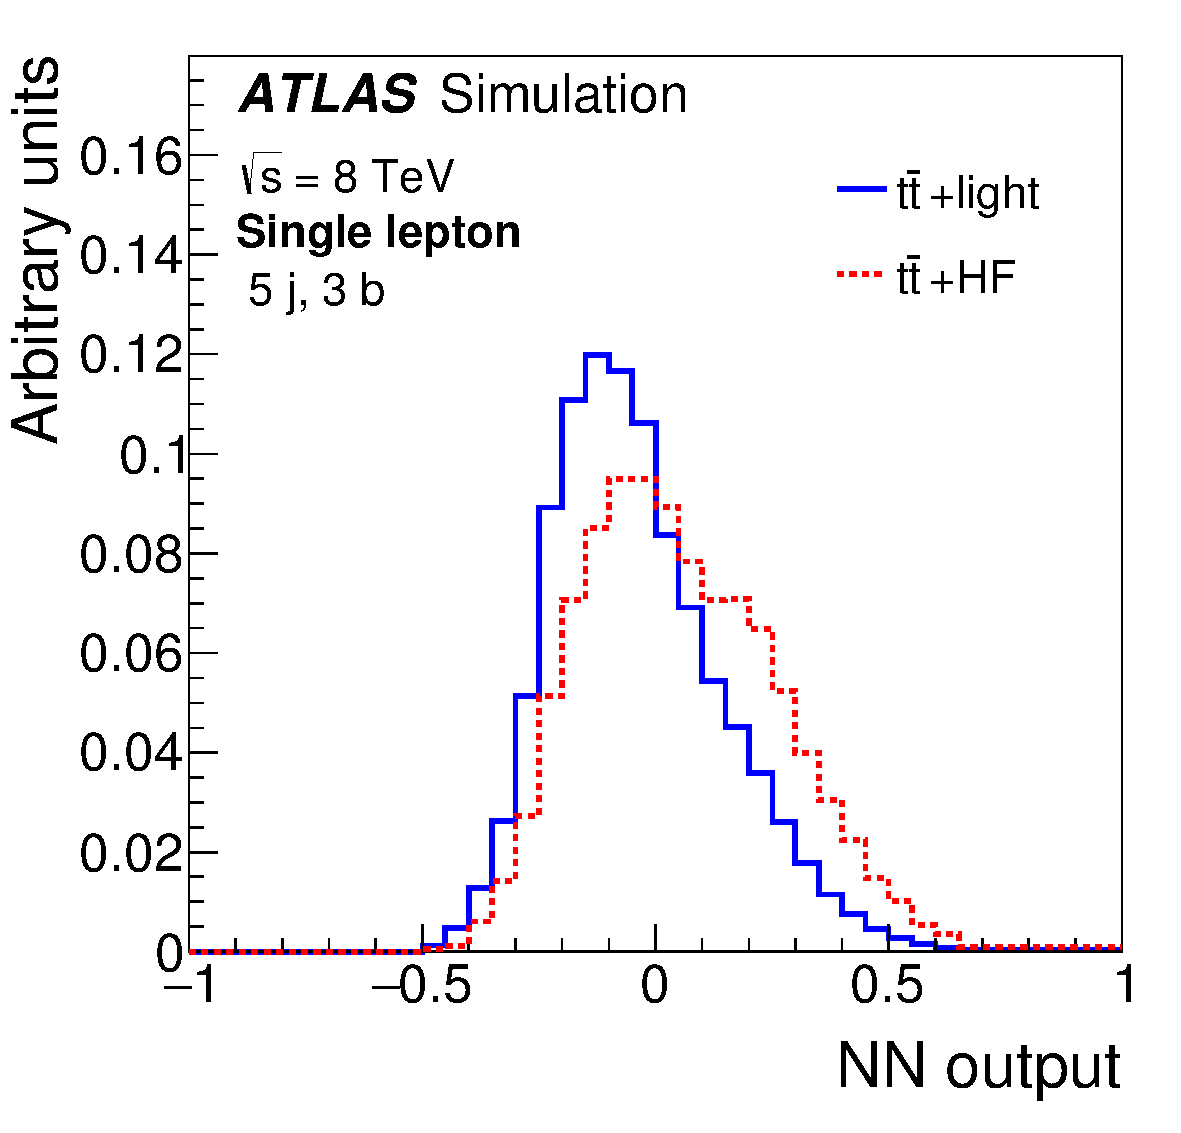
\includegraphics[width=\textwidth]{Analysis/Figures_ttH/NN125_5j_3b_kin_5_flav.pdf}\label{fig:Discriminationlj_a}
\caption{}\end{subfigure}
\begin{subfigure}{0.49\textwidth}
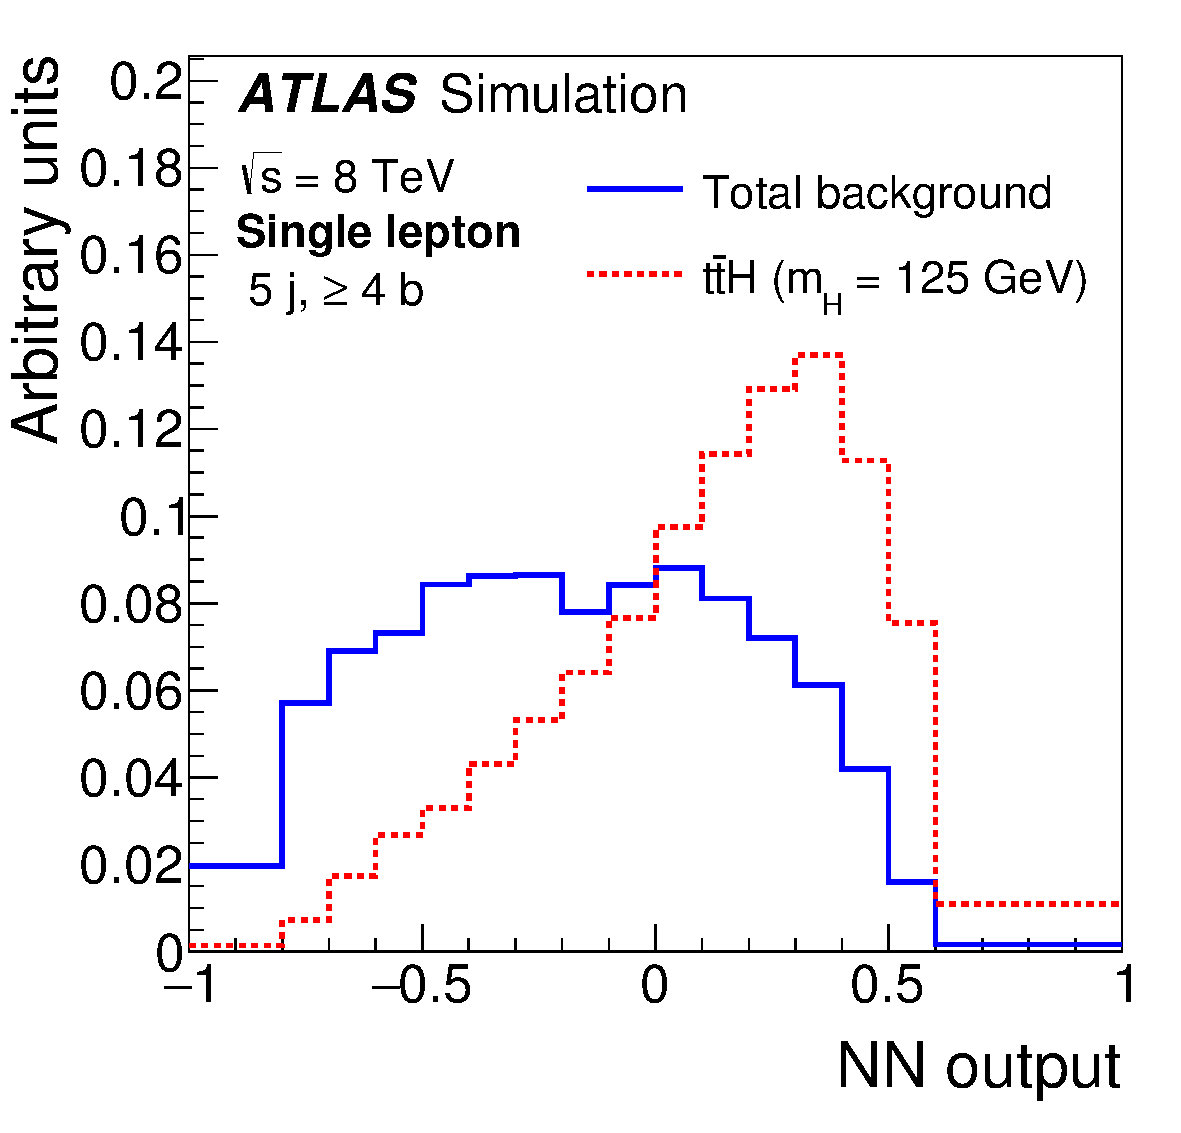
\includegraphics[width=\textwidth]{Analysis/Figures_ttH/NN125_5j_ge4b_kin_5_sep.pdf}\label{fig:Discriminationlj_b}\\
\caption{}\end{subfigure}
\begin{subfigure}{0.49\textwidth}
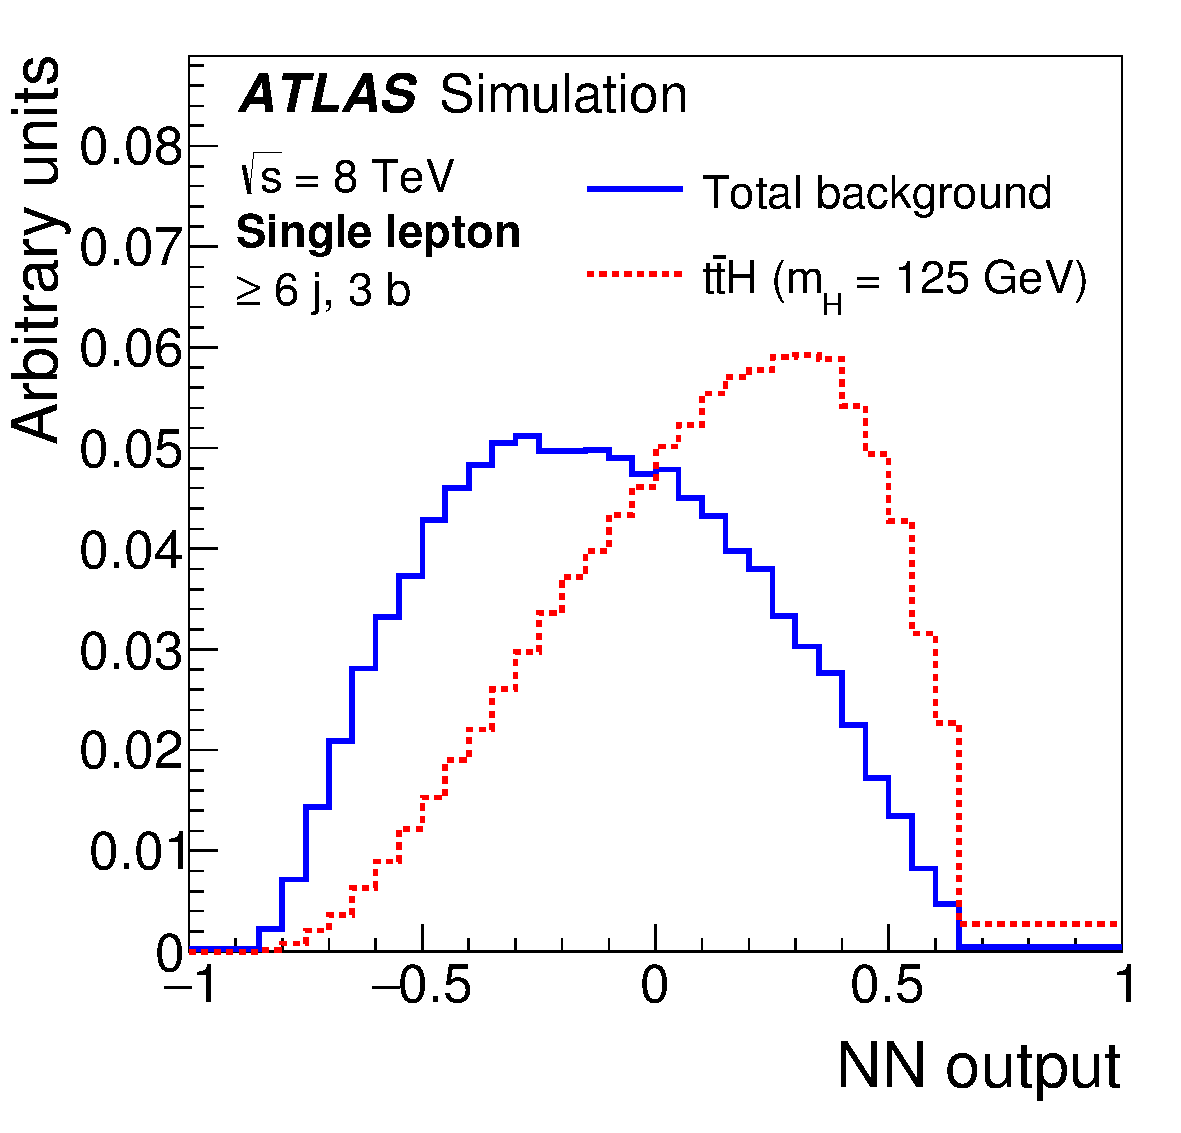
\includegraphics[width=\textwidth]{Analysis/Figures_ttH/NN125_6j_3b_kin_ME_6jincl_sep.pdf}\label{fig:Discriminationlj_c}
\caption{}\end{subfigure}
\begin{subfigure}{0.49\textwidth}
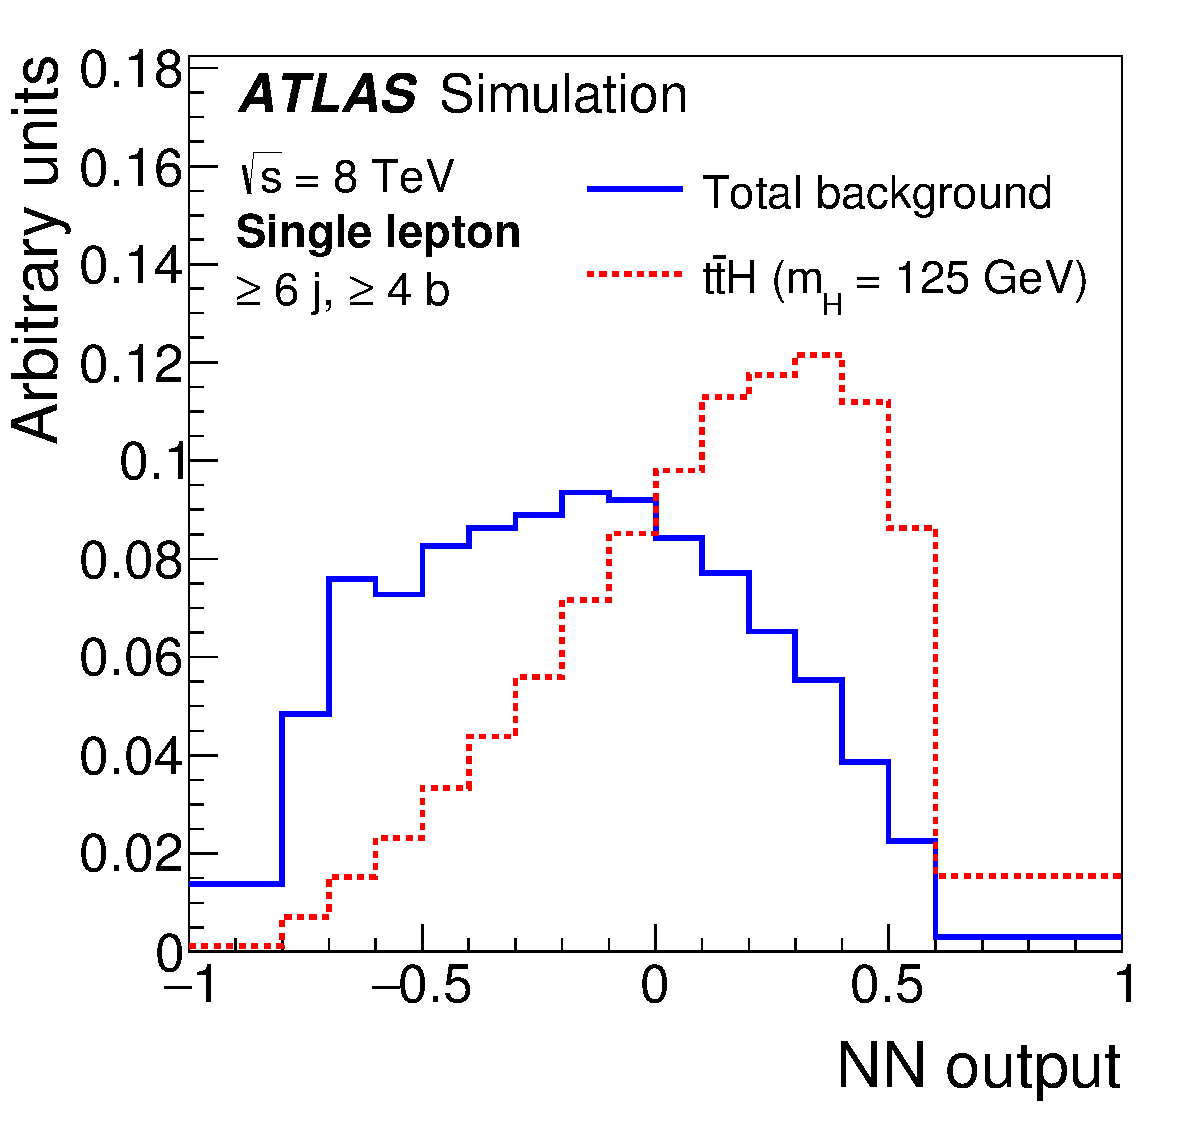
\includegraphics[width=\textwidth]{Analysis/Figures_ttH/NN125_6j_ge4b_kin_ME_6jincl_sep.pdf}\label{fig:Discriminationlj_d}
\caption{}\end{subfigure}
\caption{NN output for the different regions: (a) \fivethree, (b) \fivefour, (c) \sixthree\ and (d) \sixfour.
  In the \fivethree\ region the \ttbar+HF production is considered as signal and \ttbar+light as background
whereas in the rest of the regions the NN is trained to separate the \tth\ signal 
from the total background.  The distributions are normalized to unit area. }
\label{fig:Discriminationlj}
\end{figure}

